\section{Résultats}
\label{sec:4}

\subsection{Base générée}
\label{sec:4.1}

La base principale est générée sur le réseau ISOMORPH d'origine, dans la représentation par flux, au niveau de tension 75 : la sévérité varie de 0,68 à 1, la durée des perturbations de 8 à 24 jours et le taux de tension de 1,08 à 1,42. Les seuils critiques des profils sont relevés à 0,98, 0,95 et 0,92, car avec un taux de service minimal médian proche de 0,87, les seuils nominaux laissaient les profils prudent et tardif presque toujours inactifs ; l'ordre des profils, seul objet de la comparaison, est conservé.

La base compte 2 000 scénarios, soit 8 000 versions de crise, également réparties entre les cinq natures. L'ajustement est satisfaisant (coefficient de détermination médian de 0,88) et la perte cumulée IPC est très fidèle au service effectivement perdu (corrélation de 0,97), ce qui en fait l'indicateur principal (\voirSM{S5.1}).

\subsection{Effet des politiques de gestion}
\label{sec:4.2}

Le tableau~\ref{tab:d12} compare les quatre versions de chaque crise.

\begin{table*}[htbp]
\caption{Réaction et résilience selon la politique de gestion (2 000 crises).}
\label{tab:d12}
\footnotesize
\begin{tabularx}{\textwidth}{@{}LP{2.3cm}P{2.3cm}P{2.3cm}P{2.3cm}@{}}
\toprule
\textbf{Indicateur} & \textbf{Sans réaction} & \textbf{Réactif} & \textbf{Prudent} & \textbf{Tardif} \\
\midrule
Versions avec au moins un levier engagé & sans objet & 98 \% & 88 \% & 56 \% \\
Leviers engagés en moyenne & 0 & 2,8 & 2,0 & 0,7 \\
Détection, jours après le début (médiane) & sans objet & 0 & 1 & 3 \\
Taux de service minimal (médiane) & 0,87 & 0,89 & 0,88 & 0,87 \\
Retour à la normale, jours après le début (médiane) & 14 & 4 & 11 & 13 \\
IPC, médiane [quartiles] & 0,67 [0,43 ; 1,02] & 0,11 [0,07 ; 0,18] & 0,51 [0,36 ; 0,69] & 0,58 [0,43 ; 0,74] \\
Part du service perdu évitée & référence & 73 \% & 18 \% & 14 \% \\
\bottomrule
\end{tabularx}
\end{table*}

La réactivité domine. Le profil réactif réduit la perte cumulée de 82~\% en médiane par rapport à l'absence de réaction, contre 17~\% pour le profil prudent et 0~\% pour le profil tardif, dont la moitié des crises ne déclenchent aucune action ; les trois écarts sont significatifs (test des rangs signés de Wilcoxon apparié, $p < 10^{-150}$). Les leviers n'ayant pas de coût dans le modèle, agir plus tôt n'a jamais d'inconvénient, et cette domination est en partie structurelle.

Le taux de service minimal est en revanche presque identique d'un profil à l'autre : aucune politique n'empêche la chute, et la différence tient à sa durée (Fig.~\ref{fig:d5}). Le retour à la normale intervient au quatrième jour pour le profil réactif, contre le quatorzième sans réaction. La perte cumulée du profil réactif devient ainsi indépendante de la durée du choc (corrélation de rangs de Spearman de 0,01), alors qu'elle en dépend nettement sans réaction (0,48). La sévérité pèse peu sur la perte (0,08) : c'est la persistance du choc, non son intensité, qui fait la crise.

\begin{center}
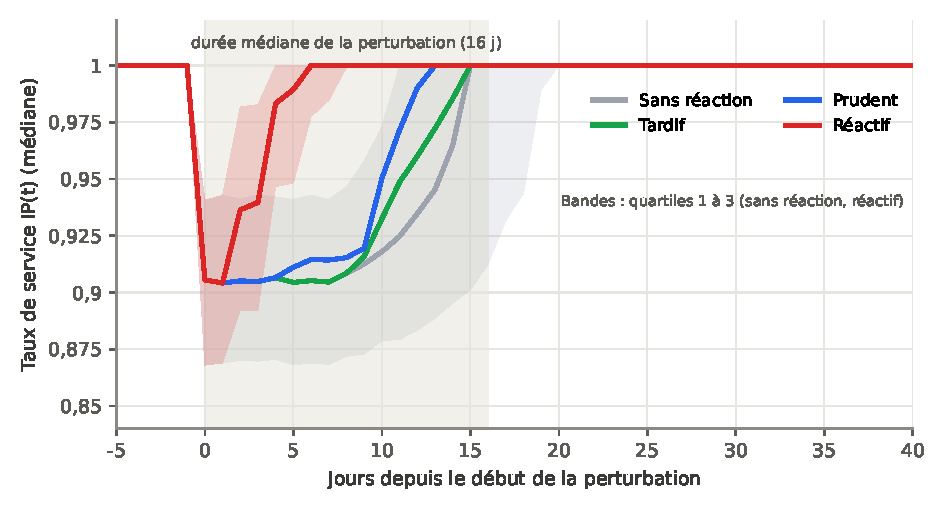
\includegraphics[width=0.62\textwidth]{figures/Fig5_trajectoire_mediane.pdf}
\captionof{figure}{Trajectoire médiane du taux de service selon la politique de gestion (2 000 crises recalées sur le début de la perturbation).}\label{fig:d5}
\end{center}

L'efficacité des politiques dépend de la nature du choc : le profil prudent est sans effet sur une panne fournisseur mais réduit de 41~\% la perte d'une congestion (\voirSM{S5.2}). En classant la perte en trois niveaux de même effectif, le profil prudent atteint le même niveau que le profil réactif dans 18~\% des crises, et cette proportion atteint 31~\% pour les perturbations de 12 jours au plus contre 11~\% au-delà de 18 jours : une crise courte peut être gérée sobrement, une crise longue exige de la réactivité.

Un lot de contrôle de 500 scénarios sur le réseau paramétrique confirme ces proportions : la part du service perdu évitée y atteint 67~\%, 17~\% et 13~\% pour les profils réactif, prudent et tardif. La topologie modifie en revanche l'efficacité des leviers : sur ce réseau aux voies de secours étroites, le profil réactif ne réduit plus que de 25~\% la perte d'une coupure de lien et de 53~\% celle d'une fermeture, contre 73~\% et 82~\% sur ISOMORPH.

\subsection{Pronostic, diagnostic et préconisation}
\label{sec:4.3}

La structure apprise (Fig.~\ref{fig:d6}) compte 41 arcs, sans aucun arc contraire à l'ordre des paliers, et retrouve le mécanisme précédent : la perte cumulée dépend directement de la politique, de la profondeur $h$ et de la durée $d$ du palier, et cette durée dépend de la politique, de la durée de la perturbation et du délai de réaction.

\begin{center}
\resizebox{0.85\textwidth}{!}{% Figure : réseau bayésien appris sous contraintes, avec la distribution marginale de chaque variable
% (données : fichier .bif exporté par BayesArtist ; marginales obtenues par inférence exacte sans observation)
\begin{tikzpicture}[
  bx/.style={draw=#1, fill=#1!10, rounded corners=3pt, minimum width=3.25cm, inner sep=0pt},
  tt/.style={font=\scriptsize\bfseries, text=black!80, anchor=north, align=center, inner sep=1pt},
  ml/.style={font=\tiny, anchor=west, inner sep=0pt},
  pc/.style={font=\tiny, anchor=east, inner sep=0pt},
  a/.style={-{Stealth[length=1.4mm]}, black!30, thin},
  m/.style={-{Stealth[length=2mm]}, polreac, very thick}]
  \node[font=\small\bfseries, text=black!70] at (0.00,6.56) {Contexte};
  % cible
  \node[bx=palctx, minimum height=1.360cm] (cible) at (0.00,3.945) {};
  \node[tt] at (0.00,4.585) {Position de la cible};
  \node[ml] at (-1.53,4.060) {Passage obligé};
  \fill[black!8] (0.095,3.975) rectangle (0.815,4.145);
  \fill[palctx] (0.095,3.975) rectangle (0.137,4.145);
  \node[pc] at (1.54,4.060) {5,8\,\%};
  \node[ml] at (-1.53,3.770) {Site redondé};
  \fill[black!8] (0.095,3.685) rectangle (0.815,3.855);
  \fill[palctx] (0.095,3.685) rectangle (0.488,3.855);
  \node[pc] at (1.54,3.770) {54,6\,\%};
  \node[ml] at (-1.53,3.480) {Réseau entier};
  \fill[black!8] (0.095,3.395) rectangle (0.815,3.565);
  \fill[palctx] (0.095,3.395) rectangle (0.380,3.565);
  \node[pc] at (1.54,3.480) {39,6\,\%};
  % partcrit
  \node[bx=palctx, minimum height=1.630cm] (partcrit) at (0.00,2.050) {};
  \node[tt] at (0.00,2.825) {Part des articles\\critiques};
  \node[ml] at (-1.53,2.030) {Faible};
  \fill[black!8] (0.095,1.945) rectangle (0.815,2.115);
  \fill[palctx] (0.095,1.945) rectangle (0.335,2.115);
  \node[pc] at (1.54,2.030) {33,4\,\%};
  \node[ml] at (-1.53,1.740) {Moyen};
  \fill[black!8] (0.095,1.655) rectangle (0.815,1.825);
  \fill[palctx] (0.095,1.655) rectangle (0.335,1.825);
  \node[pc] at (1.54,1.740) {33,4\,\%};
  \node[ml] at (-1.53,1.450) {Fort};
  \fill[black!8] (0.095,1.365) rectangle (0.815,1.535);
  \fill[palctx] (0.095,1.365) rectangle (0.334,1.535);
  \node[pc] at (1.54,1.450) {33,2\,\%};
  % nature
  \node[bx=palctx, minimum height=1.940cm] (nature) at (0.00,-0.135) {};
  \node[tt] at (0.00,0.795) {Nature};
  \node[ml] at (-1.53,0.270) {Panne fourn.};
  \fill[black!8] (0.095,0.185) rectangle (0.815,0.355);
  \fill[palctx] (0.095,0.185) rectangle (0.250,0.355);
  \node[pc] at (1.54,0.270) {21,5\,\%};
  \node[ml] at (-1.53,-0.020) {Coupure lien};
  \fill[black!8] (0.095,-0.105) rectangle (0.815,0.065);
  \fill[palctx] (0.095,-0.105) rectangle (0.233,0.065);
  \node[pc] at (1.54,-0.020) {19,1\,\%};
  \node[ml] at (-1.53,-0.310) {Fermeture site};
  \fill[black!8] (0.095,-0.395) rectangle (0.815,-0.225);
  \fill[palctx] (0.095,-0.395) rectangle (0.238,-0.225);
  \node[pc] at (1.54,-0.310) {19,8\,\%};
  \node[ml] at (-1.53,-0.600) {Pic demande};
  \fill[black!8] (0.095,-0.685) rectangle (0.815,-0.515);
  \fill[palctx] (0.095,-0.685) rectangle (0.241,-0.515);
  \node[pc] at (1.54,-0.600) {20,3\,\%};
  \node[ml] at (-1.53,-0.890) {Congestion};
  \fill[black!8] (0.095,-0.975) rectangle (0.815,-0.805);
  \fill[palctx] (0.095,-0.975) rectangle (0.235,-0.805);
  \node[pc] at (1.54,-0.890) {19,4\,\%};
  % severite
  \node[bx=palctx, minimum height=1.360cm] (severite) at (0.00,-2.185) {};
  \node[tt] at (0.00,-1.545) {Sévérité};
  \node[ml] at (-1.53,-2.070) {Faible};
  \fill[black!8] (0.095,-2.155) rectangle (0.815,-1.985);
  \fill[palctx] (0.095,-2.155) rectangle (0.335,-1.985);
  \node[pc] at (1.54,-2.070) {33,4\,\%};
  \node[ml] at (-1.53,-2.360) {Moyen};
  \fill[black!8] (0.095,-2.445) rectangle (0.815,-2.275);
  \fill[palctx] (0.095,-2.445) rectangle (0.335,-2.275);
  \node[pc] at (1.54,-2.360) {33,4\,\%};
  \node[ml] at (-1.53,-2.650) {Fort};
  \fill[black!8] (0.095,-2.735) rectangle (0.815,-2.565);
  \fill[palctx] (0.095,-2.735) rectangle (0.334,-2.565);
  \node[pc] at (1.54,-2.650) {33,2\,\%};
  % duree
  \node[bx=palctx, minimum height=1.360cm] (duree) at (0.00,-3.945) {};
  \node[tt] at (0.00,-3.305) {Durée};
  \node[ml] at (-1.53,-3.830) {Faible};
  \fill[black!8] (0.095,-3.915) rectangle (0.815,-3.745);
  \fill[palctx] (0.095,-3.915) rectangle (0.346,-3.745);
  \node[pc] at (1.54,-3.830) {34,8\,\%};
  \node[ml] at (-1.53,-4.120) {Moyen};
  \fill[black!8] (0.095,-4.205) rectangle (0.815,-4.035);
  \fill[palctx] (0.095,-4.205) rectangle (0.328,-4.035);
  \node[pc] at (1.54,-4.120) {32,3\,\%};
  \node[ml] at (-1.53,-4.410) {Fort};
  \fill[black!8] (0.095,-4.495) rectangle (0.815,-4.325);
  \fill[palctx] (0.095,-4.495) rectangle (0.332,-4.325);
  \node[pc] at (1.54,-4.410) {32,9\,\%};
  \node[font=\small\bfseries, text=black!70] at (4.00,6.56) {Politique};
  % profil
  \node[bx=palpol, minimum height=1.650cm] (profil) at (4.00,0.000) {};
  \node[tt] at (4.00,0.785) {Profil de gestion};
  \node[ml] at (2.46,0.260) {Sans réaction};
  \fill[black!8] (4.095,0.175) rectangle (4.815,0.345);
  \fill[palpol] (4.095,0.175) rectangle (4.275,0.345);
  \node[pc] at (5.54,0.260) {25,0\,\%};
  \node[ml] at (2.46,-0.030) {Réactif};
  \fill[black!8] (4.095,-0.115) rectangle (4.815,0.055);
  \fill[palpol] (4.095,-0.115) rectangle (4.275,0.055);
  \node[pc] at (5.54,-0.030) {25,0\,\%};
  \node[ml] at (2.46,-0.320) {Prudent};
  \fill[black!8] (4.095,-0.405) rectangle (4.815,-0.235);
  \fill[palpol] (4.095,-0.405) rectangle (4.275,-0.235);
  \node[pc] at (5.54,-0.320) {25,0\,\%};
  \node[ml] at (2.46,-0.610) {Tardif};
  \fill[black!8] (4.095,-0.695) rectangle (4.815,-0.525);
  \fill[palpol] (4.095,-0.695) rectangle (4.275,-0.525);
  \node[pc] at (5.54,-0.610) {25,0\,\%};
  \node[font=\small\bfseries, text=black!70] at (8.00,6.56) {Réponse};
  % detection
  \node[bx=palrep, minimum height=1.940cm] (detection) at (8.00,4.990) {};
  \node[tt] at (8.00,5.920) {Détection};
  \node[ml] at (6.46,5.395) {J0};
  \fill[black!8] (8.095,5.310) rectangle (8.815,5.480);
  \fill[palrep] (8.095,5.310) rectangle (8.262,5.480);
  \node[pc] at (9.54,5.395) {23,2\,\%};
  \node[ml] at (6.46,5.105) {J1 à J2};
  \fill[black!8] (8.095,5.020) rectangle (8.815,5.190);
  \fill[palrep] (8.095,5.020) rectangle (8.243,5.190);
  \node[pc] at (9.54,5.105) {20,6\,\%};
  \node[ml] at (6.46,4.815) {J3 et plus};
  \fill[black!8] (8.095,4.730) rectangle (8.815,4.900);
  \fill[palrep] (8.095,4.730) rectangle (8.216,4.900);
  \node[pc] at (9.54,4.815) {16,8\,\%};
  \node[ml] at (6.46,4.525) {Non détectée};
  \fill[black!8] (8.095,4.440) rectangle (8.815,4.610);
  \fill[palrep] (8.095,4.440) rectangle (8.199,4.610);
  \node[pc] at (9.54,4.525) {14,4\,\%};
  \node[ml] at (6.46,4.235) {Sans objet};
  \fill[black!8] (8.095,4.150) rectangle (8.815,4.320);
  \fill[palrep] (8.095,4.150) rectangle (8.275,4.320);
  \node[pc] at (9.54,4.235) {25,0\,\%};
  % nbleviers
  \node[bx=palrep, minimum height=1.650cm] (nbleviers) at (8.00,2.795) {};
  \node[tt] at (8.00,3.580) {Nombre de leviers};
  \node[ml] at (6.46,3.055) {0};
  \fill[black!8] (8.095,2.970) rectangle (8.815,3.140);
  \fill[palrep] (8.095,2.970) rectangle (8.377,3.140);
  \node[pc] at (9.54,3.055) {39,2\,\%};
  \node[ml] at (6.46,2.765) {1};
  \fill[black!8] (8.095,2.680) rectangle (8.815,2.850);
  \fill[palrep] (8.095,2.680) rectangle (8.213,2.850);
  \node[pc] at (9.54,2.765) {16,4\,\%};
  \node[ml] at (6.46,2.475) {2};
  \fill[black!8] (8.095,2.390) rectangle (8.815,2.560);
  \fill[palrep] (8.095,2.390) rectangle (8.263,2.560);
  \node[pc] at (9.54,2.475) {23,3\,\%};
  \node[ml] at (6.46,2.185) {3 et plus};
  \fill[black!8] (8.095,2.100) rectangle (8.815,2.270);
  \fill[palrep] (8.095,2.100) rectangle (8.248,2.270);
  \node[pc] at (9.54,2.185) {21,2\,\%};
  % lag
  \node[bx=palrep, minimum height=1.650cm] (lag) at (8.00,0.745) {};
  \node[tt] at (8.00,1.530) {Délai de réaction};
  \node[ml] at (6.46,1.005) {Court};
  \fill[black!8] (8.095,0.920) rectangle (8.815,1.090);
  \fill[palrep] (8.095,0.920) rectangle (8.257,1.090);
  \node[pc] at (9.54,1.005) {22,5\,\%};
  \node[ml] at (6.46,0.715) {Moyen};
  \fill[black!8] (8.095,0.630) rectangle (8.815,0.800);
  \fill[palrep] (8.095,0.630) rectangle (8.278,0.800);
  \node[pc] at (9.54,0.715) {25,4\,\%};
  \node[ml] at (6.46,0.425) {Long};
  \fill[black!8] (8.095,0.340) rectangle (8.815,0.510);
  \fill[palrep] (8.095,0.340) rectangle (8.187,0.510);
  \node[pc] at (9.54,0.425) {12,8\,\%};
  \node[ml] at (6.46,0.135) {Sans objet};
  \fill[black!8] (8.095,0.050) rectangle (8.815,0.220);
  \fill[palrep] (8.095,0.050) rectangle (8.377,0.220);
  \node[pc] at (9.54,0.135) {39,2\,\%};
  % fstock
  \node[bx=palrep, minimum height=1.070cm] (fstock) at (8.00,-1.015) {};
  \node[tt] at (8.00,-0.520) {Leviers de stock};
  \node[ml] at (6.46,-1.045) {Non};
  \fill[black!8] (8.095,-1.130) rectangle (8.815,-0.960);
  \fill[palrep] (8.095,-1.130) rectangle (8.641,-0.960);
  \node[pc] at (9.54,-1.045) {75,8\,\%};
  \node[ml] at (6.46,-1.335) {Oui};
  \fill[black!8] (8.095,-1.420) rectangle (8.815,-1.250);
  \fill[palrep] (8.095,-1.420) rectangle (8.269,-1.250);
  \node[pc] at (9.54,-1.335) {24,2\,\%};
  % freroutage
  \node[bx=palrep, minimum height=1.070cm] (freroutage) at (8.00,-2.485) {};
  \node[tt] at (8.00,-1.990) {Leviers de reroutage};
  \node[ml] at (6.46,-2.515) {Non};
  \fill[black!8] (8.095,-2.600) rectangle (8.815,-2.430);
  \fill[palrep] (8.095,-2.600) rectangle (8.650,-2.430);
  \node[pc] at (9.54,-2.515) {77,1\,\%};
  \node[ml] at (6.46,-2.805) {Oui};
  \fill[black!8] (8.095,-2.890) rectangle (8.815,-2.720);
  \fill[palrep] (8.095,-2.890) rectangle (8.260,-2.720);
  \node[pc] at (9.54,-2.805) {22,9\,\%};
  % fcapacite
  \node[bx=palrep, minimum height=1.070cm] (fcapacite) at (8.00,-3.955) {};
  \node[tt] at (8.00,-3.460) {Leviers de capacité};
  \node[ml] at (6.46,-3.985) {Non};
  \fill[black!8] (8.095,-4.070) rectangle (8.815,-3.900);
  \fill[palrep] (8.095,-4.070) rectangle (8.586,-3.900);
  \node[pc] at (9.54,-3.985) {68,2\,\%};
  \node[ml] at (6.46,-4.275) {Oui};
  \fill[black!8] (8.095,-4.360) rectangle (8.815,-4.190);
  \fill[palrep] (8.095,-4.360) rectangle (8.324,-4.190);
  \node[pc] at (9.54,-4.275) {31,8\,\%};
  % fdemande
  \node[bx=palrep, minimum height=1.070cm] (fdemande) at (8.00,-5.425) {};
  \node[tt] at (8.00,-4.930) {Leviers de demande};
  \node[ml] at (6.46,-5.455) {Non};
  \fill[black!8] (8.095,-5.540) rectangle (8.815,-5.370);
  \fill[palrep] (8.095,-5.540) rectangle (8.628,-5.370);
  \node[pc] at (9.54,-5.455) {74,0\,\%};
  \node[ml] at (6.46,-5.745) {Oui};
  \fill[black!8] (8.095,-5.830) rectangle (8.815,-5.660);
  \fill[palrep] (8.095,-5.830) rectangle (8.282,-5.660);
  \node[pc] at (9.54,-5.745) {26,0\,\%};
  \node[font=\small\bfseries, text=black!70] at (12.00,6.56) {Mécanisme};
  % beta
  \node[bx=palmec, minimum height=1.360cm] (beta) at (12.00,2.640) {};
  \node[tt] at (12.00,3.280) {$\beta$ (reprise)};
  \node[ml] at (10.46,2.755) {Faible};
  \fill[black!8] (12.095,2.670) rectangle (12.815,2.840);
  \fill[palmec] (12.095,2.670) rectangle (12.337,2.840);
  \node[pc] at (13.54,2.755) {33,6\,\%};
  \node[ml] at (10.46,2.465) {Moyen};
  \fill[black!8] (12.095,2.380) rectangle (12.815,2.550);
  \fill[palmec] (12.095,2.380) rectangle (12.331,2.550);
  \node[pc] at (13.54,2.465) {32,8\,\%};
  \node[ml] at (10.46,2.175) {Fort};
  \fill[black!8] (12.095,2.090) rectangle (12.815,2.260);
  \fill[palmec] (12.095,2.090) rectangle (12.337,2.260);
  \node[pc] at (13.54,2.175) {33,6\,\%};
  % h
  \node[bx=palmec, minimum height=1.360cm] (h) at (12.00,0.880) {};
  \node[tt] at (12.00,1.520) {$h$ (profondeur)};
  \node[ml] at (10.46,0.995) {Faible};
  \fill[black!8] (12.095,0.910) rectangle (12.815,1.080);
  \fill[palmec] (12.095,0.910) rectangle (12.338,1.080);
  \node[pc] at (13.54,0.995) {33,7\,\%};
  \node[ml] at (10.46,0.705) {Moyen};
  \fill[black!8] (12.095,0.620) rectangle (12.815,0.790);
  \fill[palmec] (12.095,0.620) rectangle (12.335,0.790);
  \node[pc] at (13.54,0.705) {33,4\,\%};
  \node[ml] at (10.46,0.415) {Fort};
  \fill[black!8] (12.095,0.330) rectangle (12.815,0.500);
  \fill[palmec] (12.095,0.330) rectangle (12.331,0.500);
  \node[pc] at (13.54,0.415) {32,8\,\%};
  % alpha
  \node[bx=palmec, minimum height=1.360cm] (alpha) at (12.00,-0.880) {};
  \node[tt] at (12.00,-0.240) {$\alpha$ (chute)};
  \node[ml] at (10.46,-0.765) {Faible};
  \fill[black!8] (12.095,-0.850) rectangle (12.815,-0.680);
  \fill[palmec] (12.095,-0.850) rectangle (12.334,-0.680);
  \node[pc] at (13.54,-0.765) {33,2\,\%};
  \node[ml] at (10.46,-1.055) {Moyen};
  \fill[black!8] (12.095,-1.140) rectangle (12.815,-0.970);
  \fill[palmec] (12.095,-1.140) rectangle (12.335,-0.970);
  \node[pc] at (13.54,-1.055) {33,3\,\%};
  \node[ml] at (10.46,-1.345) {Fort};
  \fill[black!8] (12.095,-1.430) rectangle (12.815,-1.260);
  \fill[palmec] (12.095,-1.430) rectangle (12.335,-1.260);
  \node[pc] at (13.54,-1.345) {33,4\,\%};
  % d
  \node[bx=palmec, minimum height=1.360cm] (d) at (12.00,-2.640) {};
  \node[tt] at (12.00,-2.000) {$d$ (durée du palier)};
  \node[ml] at (10.46,-2.525) {Faible};
  \fill[black!8] (12.095,-2.610) rectangle (12.815,-2.440);
  \fill[palmec] (12.095,-2.610) rectangle (12.338,-2.440);
  \node[pc] at (13.54,-2.525) {33,8\,\%};
  \node[ml] at (10.46,-2.815) {Moyen};
  \fill[black!8] (12.095,-2.900) rectangle (12.815,-2.730);
  \fill[palmec] (12.095,-2.900) rectangle (12.334,-2.730);
  \node[pc] at (13.54,-2.815) {33,2\,\%};
  \node[ml] at (10.46,-3.105) {Fort};
  \fill[black!8] (12.095,-3.190) rectangle (12.815,-3.020);
  \fill[palmec] (12.095,-3.190) rectangle (12.333,-3.020);
  \node[pc] at (13.54,-3.105) {33,0\,\%};
  \node[font=\small\bfseries, text=black!70] at (16.00,6.56) {Résilience};
  % CRD
  \node[bx=palres, minimum height=1.360cm] (CRD) at (16.00,1.760) {};
  \node[tt] at (16.00,2.400) {CRD};
  \node[ml] at (14.46,1.875) {Faible};
  \fill[black!8] (16.095,1.790) rectangle (16.815,1.960);
  \fill[palres] (16.095,1.790) rectangle (16.345,1.960);
  \node[pc] at (17.55,1.875) {34,7\,\%};
  \node[ml] at (14.46,1.585) {Moyen};
  \fill[black!8] (16.095,1.500) rectangle (16.815,1.670);
  \fill[palres] (16.095,1.500) rectangle (16.320,1.670);
  \node[pc] at (17.55,1.585) {31,3\,\%};
  \node[ml] at (14.46,1.295) {Fort};
  \fill[black!8] (16.095,1.210) rectangle (16.815,1.380);
  \fill[palres] (16.095,1.210) rectangle (16.340,1.380);
  \node[pc] at (17.55,1.295) {34,0\,\%};
  % IPC
  \node[bx=palres, minimum height=1.360cm] (IPC) at (16.00,0.000) {};
  \node[tt] at (16.00,0.640) {IPC};
  \node[ml] at (14.46,0.115) {Faible};
  \fill[black!8] (16.095,0.030) rectangle (16.815,0.200);
  \fill[palres] (16.095,0.030) rectangle (16.341,0.200);
  \node[pc] at (17.55,0.115) {34,1\,\%};
  \node[ml] at (14.46,-0.175) {Moyen};
  \fill[black!8] (16.095,-0.260) rectangle (16.815,-0.090);
  \fill[palres] (16.095,-0.260) rectangle (16.333,-0.090);
  \node[pc] at (17.55,-0.175) {33,0\,\%};
  \node[ml] at (14.46,-0.465) {Fort};
  \fill[black!8] (16.095,-0.550) rectangle (16.815,-0.380);
  \fill[palres] (16.095,-0.550) rectangle (16.332,-0.380);
  \node[pc] at (17.55,-0.465) {32,9\,\%};
  % TRP
  \node[bx=palres, minimum height=1.360cm] (TRP) at (16.00,-1.760) {};
  \node[tt] at (16.00,-1.120) {TRP};
  \node[ml] at (14.46,-1.645) {Faible};
  \fill[black!8] (16.095,-1.730) rectangle (16.815,-1.560);
  \fill[palres] (16.095,-1.730) rectangle (16.335,-1.560);
  \node[pc] at (17.55,-1.645) {33,3\,\%};
  \node[ml] at (14.46,-1.935) {Moyen};
  \fill[black!8] (16.095,-2.020) rectangle (16.815,-1.850);
  \fill[palres] (16.095,-2.020) rectangle (16.344,-1.850);
  \node[pc] at (17.55,-1.935) {34,6\,\%};
  \node[ml] at (14.46,-2.225) {Fort};
  \fill[black!8] (16.095,-2.310) rectangle (16.815,-2.140);
  \fill[palres] (16.095,-2.310) rectangle (16.326,-2.140);
  \node[pc] at (17.55,-2.225) {32,1\,\%};
  \begin{scope}[on background layer]
    \draw[a] (cible.west) to[bend right=26] (nature.west);
    \draw[a] (cible.east) -- (detection.west);
    \draw[a] (profil.east) -- (detection.west);
    \draw[a] (nature.west) to[bend right=26] (severite.west);
    \draw[a] (nature.east) -- (nbleviers.west);
    \draw[a] (detection.east) to[bend left=26] (nbleviers.east);
    \draw[a] (severite.west) to[bend right=26] (duree.west);
    \draw[a] (profil.east) -- (beta.west);
    \draw[a] (nbleviers.east) -- (beta.west);
    \draw[a] (nature.east) -- (freroutage.west);
    \draw[a] (profil.east) -- (freroutage.west);
    \draw[a] (nbleviers.east) to[bend left=26] (freroutage.east);
    \draw[a] (nature.east) -- (fdemande.west);
    \draw[a] (profil.east) -- (fdemande.west);
    \draw[a] (nbleviers.east) to[bend left=26] (fdemande.east);
    \draw[a] (beta.east) to[bend left=26] (h.east);
    \draw[a] (detection.east) -- (h.west);
    \draw[a] (fdemande.east) -- (h.west);
    \draw[a] (profil.east) -- (fstock.west);
    \draw[a] (nbleviers.east) to[bend left=26] (fstock.east);
    \draw[a] (freroutage.east) to[bend right=26] (fstock.east);
    \draw[a] (h.east) to[bend left=26] (alpha.east);
    \draw[a] (beta.east) to[bend left=26] (alpha.east);
    \draw[a] (detection.east) to[bend left=26] (lag.east);
    \draw[a] (nbleviers.east) to[bend left=26] (lag.east);
    \draw[a] (fstock.east) to[bend right=26] (lag.east);
    \draw[a] (nature.east) -- (fcapacite.west);
    \draw[a] (nbleviers.east) to[bend left=26] (fcapacite.east);
    \draw[a] (fstock.east) to[bend left=26] (fcapacite.east);
    \draw[m] (profil.east) -- (d.west);
    \draw[m] (duree.east) -- (d.west);
    \draw[m] (lag.east) -- (d.west);
    \draw[m] (profil.east) -- (IPC.west);
    \draw[m] (h.east) -- (IPC.west);
    \draw[m] (d.east) -- (IPC.west);
    \draw[a] (d.east) -- (CRD.west);
    \draw[a] (alpha.east) -- (CRD.west);
    \draw[a] (beta.east) -- (CRD.west);
    \draw[a] (duree.east) -- (TRP.west);
    \draw[a] (d.east) -- (TRP.west);
    \draw[a] (CRD.east) to[bend left=26] (TRP.east);
  \end{scope}
  \node[font=\scriptsize, text=black!65, anchor=north, text width=17cm, align=center] at (8.00,-6.21) {Trait épais : chemin principal (la politique agit sur la durée $d$ du palier dégradé, qui détermine la perte cumulée IPC). 20 variables, 41 arcs. Barres : probabilité marginale de chaque modalité.};
\end{tikzpicture}

% ANCIEN TIKZ (structure seule, sans les modalités), conservé en commentaire
% % Figure : réseau bayésien appris sous contraintes (données : fichier .bif exporté par BayesArtist)
% \begin{tikzpicture}[x=1.18cm,y=0.98cm,
%   n/.style={draw=#1, fill=#1!12, rounded corners=3pt, font=\scriptsize, align=center, minimum width=1.9cm, minimum height=0.72cm, inner sep=1.2pt},
%   a/.style={-{Stealth[length=1.4mm]}, black!30, thin},
%   m/.style={-{Stealth[length=2mm]}, polreac, very thick}]
%   \node[font=\small\bfseries, text=black!70] at (0,5.6) {Contexte};
%   \node[n=palctx] (cible) at (0,2.700) {Position\\de la cible};
%   \node[n=palctx] (partcrit) at (0,1.350) {Part des articles\\critiques};
%   \node[n=palctx] (nature) at (0,0.000) {Nature};
%   \node[n=palctx] (severite) at (0,-1.350) {Sévérité};
%   \node[n=palctx] (duree) at (0,-2.700) {Durée};
%   \node[font=\small\bfseries, text=black!70] at (2.9,5.6) {Politique};
%   \node[n=palpol] (profil) at (2.9,0.000) {Profil de\\gestion};
%   \node[font=\small\bfseries, text=black!70] at (5.8,5.6) {Réponse};
%   \node[n=palrep] (detection) at (5.8,4.050) {Détection};
%   \node[n=palrep] (nbleviers) at (5.8,2.700) {Nombre\\de leviers};
%   \node[n=palrep] (lag) at (5.8,1.350) {Délai de\\réaction};
%   \node[n=palrep] (fstock) at (5.8,0.000) {Leviers\\de stock};
%   \node[n=palrep] (freroutage) at (5.8,-1.350) {Leviers de\\reroutage};
%   \node[n=palrep] (fcapacite) at (5.8,-2.700) {Leviers de\\capacité};
%   \node[n=palrep] (fdemande) at (5.8,-4.050) {Leviers\\de demande};
%   \node[font=\small\bfseries, text=black!70] at (8.7,5.6) {Mécanisme};
%   \node[n=palmec] (beta) at (8.7,2.025) {$\beta$ (reprise)};
%   \node[n=palmec] (h) at (8.7,0.675) {$h$ (profondeur)};
%   \node[n=palmec] (alpha) at (8.7,-0.675) {$\alpha$ (chute)};
%   \node[n=palmec] (d) at (8.7,-2.025) {$d$ (durée\\du palier)};
%   \node[font=\small\bfseries, text=black!70] at (11.6,5.6) {Résilience};
%   \node[n=palres] (CRD) at (11.6,1.350) {CRD};
%   \node[n=palres] (IPC) at (11.6,0.000) {IPC};
%   \node[n=palres] (TRP) at (11.6,-1.350) {TRP};
%   \begin{scope}[on background layer]
%     \draw[a] (cible.west) to[bend right=40] (nature.west);
%     \draw[a] (cible.east) -- (detection.west);
%     \draw[a] (profil.east) -- (detection.west);
%     \draw[a] (nature.west) to[bend right=40] (severite.west);
%     \draw[a] (nature.east) -- (nbleviers.west);
%     \draw[a] (detection.east) to[bend left=40] (nbleviers.east);
%     \draw[a] (severite.west) to[bend right=40] (duree.west);
%     \draw[a] (profil.east) -- (beta.west);
%     \draw[a] (nbleviers.east) -- (beta.west);
%     \draw[a] (nature.east) -- (freroutage.west);
%     \draw[a] (profil.east) -- (freroutage.west);
%     \draw[a] (nbleviers.east) to[bend left=40] (freroutage.east);
%     \draw[a] (nature.east) -- (fdemande.west);
%     \draw[a] (profil.east) -- (fdemande.west);
%     \draw[a] (nbleviers.east) to[bend left=40] (fdemande.east);
%     \draw[a] (beta.east) to[bend left=40] (h.east);
%     \draw[a] (detection.east) -- (h.west);
%     \draw[a] (fdemande.east) -- (h.west);
%     \draw[a] (profil.east) -- (fstock.west);
%     \draw[a] (nbleviers.east) to[bend left=40] (fstock.east);
%     \draw[a] (freroutage.east) to[bend right=40] (fstock.east);
%     \draw[a] (h.east) to[bend left=40] (alpha.east);
%     \draw[a] (beta.east) to[bend left=40] (alpha.east);
%     \draw[a] (detection.east) to[bend left=40] (lag.east);
%     \draw[a] (nbleviers.east) to[bend left=40] (lag.east);
%     \draw[a] (fstock.east) to[bend right=40] (lag.east);
%     \draw[a] (nature.east) -- (fcapacite.west);
%     \draw[a] (nbleviers.east) to[bend left=40] (fcapacite.east);
%     \draw[a] (fstock.east) to[bend left=40] (fcapacite.east);
%     \draw[m] (profil.east) -- (d.west);
%     \draw[m] (duree.east) -- (d.west);
%     \draw[m] (lag.east) -- (d.west);
%     \draw[m] (profil.east) -- (IPC.west);
%     \draw[m] (h.east) -- (IPC.west);
%     \draw[m] (d.east) -- (IPC.west);
%     \draw[a] (d.east) -- (CRD.west);
%     \draw[a] (alpha.east) -- (CRD.west);
%     \draw[a] (beta.east) -- (CRD.west);
%     \draw[a] (duree.east) -- (TRP.west);
%     \draw[a] (d.east) -- (TRP.west);
%     \draw[a] (CRD.east) to[bend left=40] (TRP.east);
%   \end{scope}
%   \node[font=\scriptsize, text=black!65, anchor=north] at (5.8,-5.1) {Trait épais : chemin principal (la politique agit sur la durée $d$ du palier dégradé, qui détermine la perte cumulée IPC). 20 variables, 41 arcs.};
% \end{tikzpicture}
}
\captionof{figure}{Réseau bayésien appris sous contraintes, variables colorées par palier de l'ordre temporel d'une crise.}\label{fig:d6}
\end{center}

Le pronostic, établi à partir des seules variables connues au moment de décider, classe correctement 65~\% des crises de test, contre 34~\% pour la classe majoritaire et 60~\% pour un modèle fondé sur la seule politique (score de Brier de 0,466 contre 0,667 et 0,494). La courbe d'apprentissage est presque plate : la limite tient à l'information disponible au moment de décider, non à la taille de la base. Le diagnostic est bien calibré pour la politique et la durée : pour les crises de test à forte perte, les probabilités a posteriori des politiques reproduisent leurs fréquences observées à 0,01 près.

Avec l'objectif d'une perte faible, seul le profil réactif réussit régulièrement, et la règle le préconise toujours. Avec l'objectif moins exigeant d'une perte qui ne soit pas forte, un arbitrage apparaît entre sécurité et sobriété, que règle le seuil $\theta$ (tableau~\ref{tab:d15}).

\begin{table*}[htbp]
\caption{Préconisation sur les crises de test, objectif d'une perte cumulée non forte.}
\label{tab:d15}
\footnotesize
\begin{tabularx}{\textwidth}{@{}LLL@{}}
\toprule
\textbf{Règle} & \textbf{Objectif atteint} & \textbf{Préconisations plus sobres que le profil réactif} \\
\midrule
Toujours le profil réactif & 99,2 \% & 0 \% \\
Réseau appris, $\theta$ = 0,9 & 99,2 \% & 0 \% \\
Réseau appris, $\theta$ = 0,8 & 97,5 \% & 15 \% \\
Réseau appris, $\theta$ = 0,7 & 86,2 \% & 37 \% \\
Réseau appris, $\theta$ = 0,6 & 69,5 \% & 84 \% \\
Référence a posteriori : politique la plus sobre ayant réussi & 99,2 \% & 67 \% \\
\bottomrule
\end{tabularx}
\end{table*}

Avec $\theta$ = 0,8, le réseau préconise une politique plus sobre dans environ une crise sur sept, pour un taux de réussite de 97,5~\%, moins de deux points sous la politique la plus interventionniste. Cette sobriété repose entièrement sur la durée prévue du choc : lorsque cette information est retirée de la description de la crise, la règle ne préconise plus aucune politique sobre. Une estimation de la durée d'une perturbation a donc une valeur décisionnelle propre. Ainsi, pour la fermeture courte d'un site redondé, le profil prudent atteint l'objectif avec une probabilité de 0,80 et devient la préconisation, alors que pour la fermeture longue d'un point de passage obligé seul le profil réactif y parvient (\voirSM{S5.3}).

La figure~\ref{fig:carte} généralise cette lecture par l'inférence à rebours, pour l'objectif d'une perte faible, aux sept contextes que la topologie d'ISOMORPH rend possibles. Le profil réactif est le plus probable partout, et d'autant plus que le choc dure : sa probabilité a posteriori passe de 0,51 à 0,58 pour un choc court à 0,72 à 0,79 pour un choc long. Pour un choc court, les autres politiques conservent chacune entre 0,12 et 0,18 : une perte faible y reste accessible sans réaction rapide.

\begin{center}
\begin{minipage}{\textwidth}\centering
% Figure : carte de préconisation par inférence à rebours sur le réseau appris, en nuage de points.
% Probabilité a posteriori de chaque profil sachant IPC = faible, pour les sept contextes (nature, position de la cible),
% un plan par durée du choc. Vert : politique la plus probable du contexte ; rouge : autres politiques.
% Valeurs identiques à l'ancienne carte (inférence exacte sur le réseau appris, fichier .bif).
\begin{tikzpicture}
\pgfplotsset{carte/.style={width=5.6cm, height=5.6cm, xmin=0.5, xmax=4.5, ymin=0, ymax=0.85,
  xtick={1,2,3,4}, xticklabels={Aucune,Tardif,Prudent,Réactif},
  ytick={0,0.2,0.4,0.6,0.8}, yticklabel style={/pgf/number format/.cd,fixed,fixed zerofill,precision=1,use comma},
  tick label style={font=\scriptsize}, label style={font=\scriptsize}, title style={font=\small\bfseries},
  ymajorgrids, grid style={gray!20}, axis lines*=left, clip=false}}
\begin{axis}[carte, title={Durée courte}, at={(0.0cm,0)}, ylabel={Probabilité a posteriori du profil}]
  \addplot[only marks, mark=*, mark size=1.8pt, appreac, fill opacity=0.75, draw opacity=0.9] coordinates {(0.73,0.16) (1.73,0.15) (2.73,0.12) (0.82,0.15) (1.82,0.14) (2.82,0.13) (0.91,0.13) (1.91,0.18) (2.91,0.17) (1.00,0.14) (2.00,0.18) (3.00,0.17) (1.09,0.14) (2.09,0.17) (3.09,0.17) (1.18,0.15) (2.18,0.15) (3.18,0.15) (1.27,0.15) (2.27,0.15) (3.27,0.15)};
  \addplot[only marks, mark=*, mark size=1.8pt, apptard, fill opacity=0.85] coordinates {(3.73,0.58) (3.82,0.57) (3.91,0.52) (4.00,0.51) (4.09,0.52) (4.18,0.55) (4.27,0.55)};
\end{axis}
\begin{axis}[carte, title={Durée moyenne}, at={(5.15cm,0)}, yticklabels={}]
  \addplot[only marks, mark=*, mark size=1.8pt, appreac, fill opacity=0.75, draw opacity=0.9] coordinates {(0.73,0.07) (1.73,0.07) (2.73,0.10) (0.82,0.06) (1.82,0.07) (2.82,0.12) (0.91,0.06) (1.91,0.10) (2.91,0.14) (1.00,0.06) (2.00,0.10) (3.00,0.14) (1.09,0.06) (2.09,0.10) (3.09,0.14) (1.18,0.07) (2.18,0.08) (3.18,0.12) (1.27,0.07) (2.27,0.08) (3.27,0.12)};
  \addplot[only marks, mark=*, mark size=1.8pt, apptard, fill opacity=0.85] coordinates {(3.73,0.76) (3.82,0.75) (3.91,0.69) (4.00,0.70) (4.09,0.70) (4.18,0.73) (4.27,0.73)};
\end{axis}
\begin{axis}[carte, title={Durée longue}, at={(10.3cm,0)}, yticklabels={}]
  \addplot[only marks, mark=*, mark size=1.8pt, appreac, fill opacity=0.75, draw opacity=0.9] coordinates {(0.73,0.06) (1.73,0.07) (2.73,0.08) (0.82,0.06) (1.82,0.07) (2.82,0.10) (0.91,0.05) (1.91,0.10) (2.91,0.13) (1.00,0.05) (2.00,0.09) (3.00,0.13) (1.09,0.05) (2.09,0.09) (3.09,0.13) (1.18,0.06) (2.18,0.08) (3.18,0.10) (1.27,0.06) (2.27,0.08) (3.27,0.10)};
  \addplot[only marks, mark=*, mark size=1.8pt, apptard, fill opacity=0.85] coordinates {(3.73,0.79) (3.82,0.77) (3.91,0.72) (4.00,0.72) (4.09,0.73) (4.18,0.76) (4.27,0.76)};
\end{axis}
\matrix[anchor=north, font=\scriptsize, column sep=4pt] at (7.6cm,-0.5cm) {
  \fill[apptard] (0,0) circle (2pt); & \node[anchor=west]{Politique la plus probable du contexte}; &
  \fill[appreac] (0,0) circle (2pt); & \node[anchor=west]{Autres politiques}; \\
};
\end{tikzpicture}

\captionof{figure}{Carte de préconisation : probabilité a posteriori de chaque profil sachant une perte cumulée faible, pour les sept contextes de nature et de position de la cible, selon la durée du choc.}\label{fig:carte}
\end{minipage}
\end{center}

\subsection{Rôle des stocks}
\label{sec:4.4}

La représentation temporelle permet d'étudier le rôle des stocks, que la base principale neutralise : 60 crises sans réaction ont été simulées sur ISOMORPH pour chaque nature et chaque couverture de stock. Pour les ruptures de distribution, la couverture agit comme un levier de robustesse progressif : plus elle est faible, plus les crises visibles sont nombreuses, de 11 à 43 sur 60 pour une coupure de lien. Le pic de demande est au contraire mieux absorbé sans stocks, le surcroît de demande devant d'abord être prélevé sur des stocks dimensionnés sur le débit nominal. La couverture de stock n'est donc pas un levier universel de résilience : elle protège contre les pertes de capacité de distribution, mais pas contre un choc de demande (\voirSM{S5.4}).

\subsection{Lecture économique}
\label{sec:4.5}

Multipliée par la demande journalière de référence, la part de service non rendue pendant les 60 jours qui suivent le choc donne les ventes perdues : une crise sans réaction coûte en moyenne 25 550 unités, soit environ 1,4 jour de demande. Le modèle ne valorisant pas les leviers, leur coût $c$ par engagement est exprimé en unités de marge $m$ : une politique est rentable tant que les ventes préservées, multipliées par $m$, couvrent le coût des leviers engagés, et le rapport $c/m$ au-delà duquel ce n'est plus le cas constitue son seuil de rentabilité (tableau~\ref{tab:eco}).

\begin{table*}[htbp]
\caption{Ventes préservées, leviers engagés et seuil de rentabilité par politique (moyennes sur 2 000 crises). Le gain marginal rapporte le surcroît de ventes préservées au surcroît de leviers par rapport à la ligne précédente.}
\label{tab:eco}
\footnotesize
\begin{tabularx}{\textwidth}{@{}LLLLLL@{}}
\toprule
\textbf{Politique} & \textbf{Ventes perdues par crise (unités)} & \textbf{Ventes préservées (unités ; part)} & \textbf{Leviers engagés par crise} & \textbf{Seuil de rentabilité ($c/m$)} & \textbf{Gain marginal par levier} \\
\midrule
Sans réaction & 25 550 & référence & 0 & sans objet & sans objet \\
Tardif & 22 020 & 3 530 ; 14~\% & 0,67 & 5 300 & 5 300 \\
Prudent & 20 980 & 4 570 ; 18~\% & 1,97 & 2 320 & 790 \\
Réactif & 7 000 & 18 550 ; 73~\% & 2,80 & 6 630 & 16 940 \\
\bottomrule
\end{tabularx}
\end{table*}

La politique réactive est à la fois la plus efficace et la plus rentable par levier : chacun de ses leviers préserve en moyenne 6 630 unités, soit environ un tiers de journée de demande. La politique prudente est au contraire économiquement dominée : elle engage plus des deux tiers des leviers de la politique réactive pour un quart de ses gains, et chaque levier qu'elle ajoute à la politique tardive ne préserve que 790 unités. Le coût d'une politique tient donc moins au nombre de leviers qu'à leur moment d'engagement.

\begin{center}
% Figure : bénéfice net moyen d'une politique par crise, selon le coût d'un levier
% (données : ip_timeseries.csv et base d'apprentissage du lot A ; calcul décrit en section 6.6)
\begin{tikzpicture}
\begin{axis}[
  width=0.93\textwidth, height=5.8cm,
  xmin=0, xmax=12000, ymin=-6, ymax=20,
  xlabel={Coût d'un levier engagé, exprimé en unités de marge ($c/m$)},
  ylabel style={align=center},
  ylabel={Bénéfice net moyen par crise\\(milliers d'unités de marge)},
  xtick={0,2000,4000,6000,8000,10000,12000},
  xticklabel style={/pgf/number format/.cd,1000 sep={\,}},
  scaled x ticks=false,
  tick label style={font=\scriptsize}, label style={font=\small},
  grid=major, grid style={black!8},
  legend style={font=\scriptsize, draw=none, fill=white, fill opacity=0.9, text opacity=1, at={(0.98,0.98)}, anchor=north east, cells={anchor=west}},
  every axis plot/.append style={line width=1.2pt}]
  \fill[appreac!6] (axis cs:0,-6) rectangle (axis cs:6628,20);
  \node[font=\scriptsize, text=appreac!85!black, anchor=south west, align=left] at (axis cs:150,-5.6) {zone où la politique\\réactive est rentable};
  \addplot[appnone] table[x=r, y expr=\thisrow{none}/1000] {figures/data/eco_benefice.dat};
  \addlegendentry{Sans réaction}
  \addplot[apptard] table[x=r, y expr=\thisrow{tardif}/1000] {figures/data/eco_benefice.dat};
  \addlegendentry{Tardif}
  \addplot[appprud] table[x=r, y expr=\thisrow{prudent}/1000] {figures/data/eco_benefice.dat};
  \addlegendentry{Prudent}
  \addplot[appreac] table[x=r, y expr=\thisrow{reactif}/1000] {figures/data/eco_benefice.dat};
  \addlegendentry{Réactif}
  \addplot[black!75, line width=1.6pt, densely dashed] table[x=r, y expr=\thisrow{posteriori}/1000] {figures/data/eco_benefice.dat};
  \addlegendentry{Meilleure politique choisie crise par crise}
  \draw[black!50, densely dotted] (axis cs:6628,-6) -- (axis cs:6628,20);
  \node[font=\scriptsize, fill=white, inner sep=1pt, anchor=west] at (axis cs:6750,9.3) {seuil de la politique réactive : 6 630};
\end{axis}
\end{tikzpicture}
\captionof{figure}{Bénéfice net moyen par crise selon le coût d'un levier. La courbe en tirets, qui choisit a posteriori la meilleure politique pour chaque crise, borne la valeur d'une préconisation adaptée.}\label{fig:eco}
\end{center}

Parmi les politiques fixes, la réactivité est optimale tant que le coût d'un levier reste sous 6 630 unités de marge ; au-delà, mieux vaut ne pas réagir (Fig.~\ref{fig:eco}). Choisir pour chaque crise la politique au meilleur bénéfice, comme si son issue était connue d'avance, porterait le bénéfice moyen de 4 560 à 8 350 unités par crise pour un levier de 5 000 unités de marge, soit 83~\% de plus que la meilleure politique fixe. Face à des perturbations mineures, en revanche, le profil réactif engage des leviers près de trente fois moins rentables que sur une crise sévère (\voirSM{S5.5}).
